\begin{figure}
\centering
    \begin{subfigure}{0.4\linewidth}
        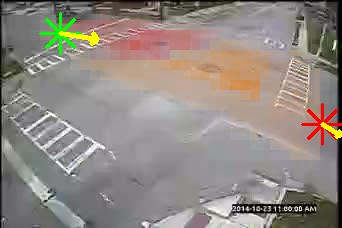
\includegraphics[width=\linewidth]{./img/semantic_tracker/193402-entry-exit-0.jpg}
        \subcaption{}
        \label{subfig:semantic-extry-exit-eg1}
    \end{subfigure}
    \begin{subfigure}{0.4\linewidth}
        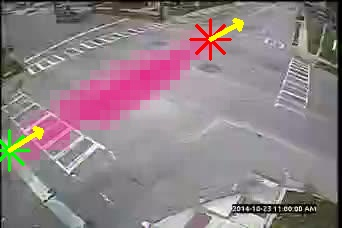
\includegraphics[width=\linewidth]{./img/semantic_tracker/193402-entry-exit-3.jpg}
        \subcaption{}
        \label{subfig:semantic-extry-exit-eg2}
    \end{subfigure}%
    \caption{Two scenarios of object enters and exits: (\subref{subfig:semantic-extry-exit-eg1}): objects enter with a tiny size and move out of image boundary; (\subref{subfig:semantic-extry-exit-eg2}): objects enter from the image boundary and exit with a tiny size in within the frame. Green and red star are the obtained entry/exit hotspots; yellow arrows shows their direction.}
    \label{fig:semantic-entry-exit}
\end{figure}